\cleardoublepage
\chapter{Text Processing and Image Retrieval}
\label{ch:text_stage}

This chapter aims at making clear how the automatic retrieval system works. Section \ref{sec:text} clarifies how the system does text processing, word extraction and how it manages to categorize the extracted data. Subsequently in section \ref{sec:retrieval} an explanation is given on how the system retrieves images for a given moment and how it is able to compare the similarity between the mined text words and the visual concepts. Lastly in section \ref{sec:diagram} a diagram that overviews the system workflow architecture is exhibited in order to clarify the process.



\section{ Word Extraction }
\label{sec:text}

In the text mining/processing stage, the query topics are analysed using Natural Language Processing tools to extract relevant words in order to retrieve the desired moment. Those words are compared with the visual concepts words obtained in the image processing stage. 

The SpaCy library \cite{Spacy2017} is used to analyse the query topics fully, extracting relevant words from the title, the description and narrative. The words extracted are divided into 10 categories being them : "relevant things", "activities", "dates", "locations", "inside", "outside", "negative relevant things", "negative activities", "negative locations" and "negative dates".

In order to assign words to each category some linguistic rules were defined,
such as semantic and syntactic rules. Semantic rules build the meaning of the
sentence from its words and how words combine syntactically. Syntax rules refer to
the rules that govern the ways in which words combine to form phrases and
sentences. 

\begin{figure}[H]
    \centering
    \captionsetup{justification=centering}
    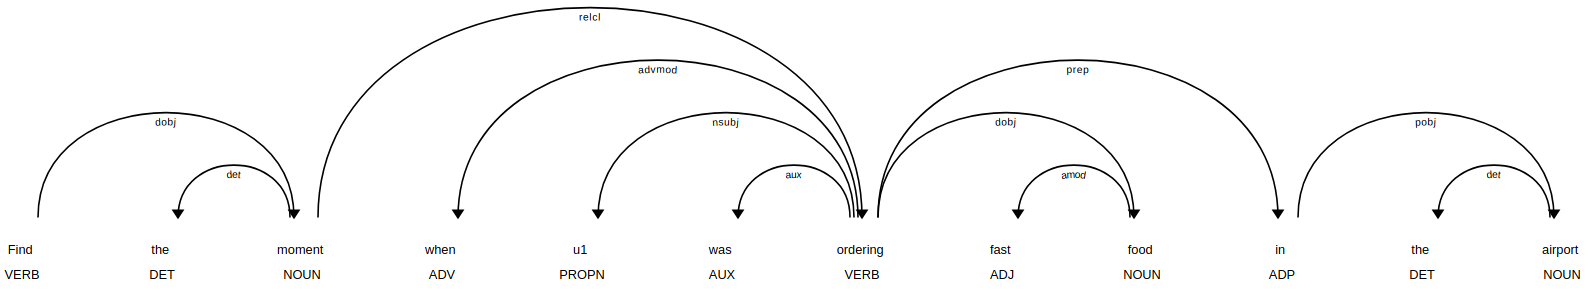
\includegraphics[width =  \textwidth]{Sections/6textprocessing/images/spacy.png}
    \caption{Linguistic annotations generated by the SpaCy library \cite{Spacy2017} for the narrative of the topic 6 of the test topics.}
    \label{fig:spacy_labels}
  \end{figure}
  
  \newpage
  
  As an example, some of the rules that were applied to the extraction and categorization of the textual data were:
  
  \begin{itemize}
    \itemsep0em
      \item  If the word is a "VERB" and ends with "ing", like "ordering" then it probably is an activity and if the words that follows are "NOUN" then those words probably refer to a location or an object.
      \item  If the word is and "ADP" (adposition) and its either "in" or "at" then the words that follow are probably locations and usually means that the moment occurs inside a location and not outside, the category "inside" is then flagged to "True" and "outside" is flagged to "False".
      \item If the word is a "NUM" (number) then it probably refers to a year.
      \item If the sentence has an auxiliary verb, the main verb usually corresponds to an activity and the words that follow the main verb may be objects or locations.
      \item If the word is an "ADJ" (adjective) then the following word is probably an object. It can also be a bi-gram like "ice cream" or in this case "fast food".
      \item If the sentence ends with "not considered relevant" the extracted words go to the negative categories.
      \item Rules for the extraction of dates, like the day of the week, the month or even years were also created. However do the the syntax of the test topics, since they had no reference to dates in the text, the dates category was discarded in order to save time. Nevertheless, for the dev topics dates were used and produced good results. As an example if in the topic it was said that the moment happened on a "wednesday" or in year 2014, only pictures from wednesday or the year 2014 were retrieved.

    \end{itemize}


Using figure \ref{fig:spacy_labels} to illustrate, the extracted words for the the narrative of the test topic 6  were:

    \begin{itemize}
        \item \textbf{relevant things} : "fast food".
        \item \textbf{activities} : "ordering", "ordering fast food".
        \item \textbf{locations} : "airport".
        \item \textbf{inside} : "True".
        \item \textbf{outside}: "False".
       
    \end{itemize}

\newpage
\section{Retrieval Stage}
\label{sec:retrieval}

    In the retrieval step the images are recovered according to the desired query topic.
    As an example figure \ref{fig:testtopic} represents the test topic number 7.
   
    \begin{figure}[H]
        \centering
        \captionsetup{justification=centering}
        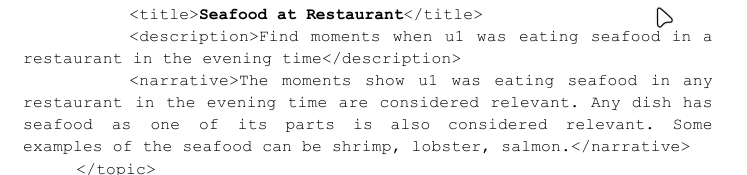
\includegraphics[width = \textwidth]{Sections/6textprocessing/images/topic.png}
        \caption{Test topic number 7.}
        \label{fig:testtopic}
      \end{figure}
      
      The extracted words of the title, description and narrative are as follows:

      \begin{itemize}
        \itemsep0em
        \item \textbf{relevant things} : 
            "seafood",
            "parts",
            "shrimp",
            "lobster",
            "salmon".
        \item \textbf{activities} : "eating",
        "eating seafood"
        \item \textbf{locations} : "restaurant",  "evening time".
        \item \textbf{inside} : "True".
        \item \textbf{outside}: "False".
        \item \textbf{dates}: NULL.
        \item \textbf{negative relevant thing}: NULL.
        \item \textbf{negative activities}: NULL.
        \item \textbf{negative locations}:  NULL.
        \item \textbf{negative dates}: NULL.
       
    \end{itemize}

    An important detail to be noticed is that the words "evening time" are wrongly placed on the locations category. One of the reasons for this to happen is because of the previously described rule, where if a word is an "ADP" and it is "in" then the following "NOUN" is probably a location, which in this case is not correct.

    \subsection{Retrieving Images According to the Similarity Between Words}

    In order to retrieve images according to the defined moment in a textual topic, a comparison is made between the extracted visual concept words from the images and the words extracted from the topics. This comparison is done trough the calculation of similarity score obtained by an NLP model.

    The SpaCy en\_core\_web\_md model allows the computer to calculate the similarity between the visual concepts and the extracted data. This model is an english multi-task CNN trained on OntoNotes, with GloVe vectors trained on Common Crawl \cite{Spacy2017} . As an example of similarity between words using the described model, the word "television" and "seafood" have a similarity of 0.0705759162558067 while "television" and "screen" have a similarity of 0.4271196001925812.
    
    A confidence score is calculated based on that value for each image and for each topic. This score ranges from a value of 0.0 (0\%) to 1.0 (100\%).

    Since the images dataset consists in 200.000 images and the test topic dataset consists on 10 topics, approximately 2.000.000 confidence score calculations had to be computed. This step is extremely exhaustive on computer time and resources, which made it  hard to make adjustments, correct errors and bugs in the code.
    
    The computation of the confidence score is also influenced by the score of the image concepts obtained trough the image processing phase. This means that an image with low prediction score has a lower confidence score. Not only is the confidence score influenced by the similarity between words, the prediction score, but also the computed weights assigned to each category. The weight for each category is obtained through two different factors, an importance weight factor and a distributed weight factor. The weight of the category is therefore the sum of the importance weight factor and the distributed weight factor.


    The distributed weight factor value is not the same for each category, the ratio of the distribution is equal to the default ratio of the importance factor of all categories. To make it clearly, if the importance weight factor for ”relevant things” is 0.5, which is half of the sum of all importance factors, and if the ”activities” category is worth 0.2 and has no extracted textual data, then half of 0.2 is distributed to ”relevant things”, which increases the importance to 0.6 and the remainder 0.1 will be distributed the same way to other categories ensuring that the sum of all importance factors and distributed weight factors is 1. The negative categories works the same way, but instead of contributing for the confidence score, it decreases the value.

    Finally, a script runs through all the selected confidence scores for a given
    query topic and stores the 50 pictures with the highest confidence score for each topic are stored and the 10 highest pictures are the ones who count for the f1@measure score.
       

    Due to the fact that the PLACES365 scene recognition model extracts scenes with very low scores, rarely above 30\%-40\% it was decided to discard the category "categories" and "attributes" from contributing to the confidence score in order to save processing time.


    In order to have a better visualization of how this calculations are done section \ref{sec:equation} shows all of the equations needed to calculate the confidence score and section \ref{sec:diagram} shows a diagram that illustrates all the steps that the system does in order to retrieve images.

  
\newpage

    \subsection{Calculation of Similarity Scores}
    Using the figures \ref{fig:image_fully_processed} and \ref{fig:image_fully_processed_resnext} to illustrate the different categories, the calculation of the similarity scores are done trough the comparision of the extracted words and the visual concepts:
    \begin{itemize}
        \itemsep0em
        \item The visual category "concepts" is compared to the textual category "relevant things";
        \item The visual category "concepts" is compared to the textual category "negative relevant things";
        \item The visual category "activity" is compared to the textual category "activities";
        \item The visual category "activity" is compared to the textual category "negative activities";
        \item The visual category "location" is compared to the textual category "locations";
        \item The visual category "location" is compared to the textual category "negative locations";
        \item "Depending if the textual category "inside" = "True" / "False" the visual category "io\_score" value will have different impact on the confidence score.
    \end{itemize}
    

    \subsection{Run 1}

    The first run to be submitted for the imageclef LMRT subtask used a combination of ResNeXt-101 and Feature Pyramid Network architectures in a basic Faster Region-based Convolutional Network (Faster R-CNN) pretrained on the COCO dataset for the extraction of visual concepts.

    In this run all of the importance weight factors for all categories were the same. This means that each category counts the same for the computation of the confidence score. No category is more important or less important. When a category is empty, their respective importance factor is equally apportionated to all other categories but never to the negative categories. If a negative category importance factor is negative, their factor is apportionated to the other negative categories. And if a positive category is empty, their factor is apportionated to the positive categories.

    Another aspect of Run 1 is that the negative categories can only impact the confidence score up to 0.5.
    
    A general threshold was previously defined in order to remove images of low
concept scores, images above the threshold are selected for the calculation of the confidence score in order to select them for the query topic.  The threshold was implemented through some trial and error during the test phases, and it merely serves the purpose of saving some computational time.

    \subsection{Run 2}

    
    In the second run, the object detection algorithm used is the YoloV3 model pretrained in the COCO dataset.  It was decided to define the importance weight factor differently for each category. It was given a bigger importance to specific categories like "relevant things" and "ioscore". Categories like ”activities” and ”locations” get a lesser importance weight factor since they are being compared to the organizers label data which is limiting and lesser accurate.  Another difference from Run 1 to Run 2 is that all of the negative categories were discarded from contributing to the confidence score, in order to save processing time and since the first results from Run 1 did not appear to impact much.
    

\newpage
\subsection{Confidence Score Computation Equations}
\label{sec:equation}
The following equations give an understanding of all the computations done in order to calculate the confidence score:






\begin{align*}
    &\textbf{ConceptScore}  =   [Weight_1]\times[HighestSimilarityScore]\times[VisualScore] \\ 
    &\textbf{LocationScore} = [Weight_2]\times[HighestSimilarityScore] \\ 
   &\textbf{ActivityScore} =  [Weight_3]\times[HighestSimilarityScore]\\
    &\textbf{InsideScore}   =  [Weight_4]\times(1-[ioscore])\\
    &\textbf{OutsideScore}  =  [Weight_5]\times([ioscore])\\
    &\textbf{PositiveScore}  =  ConceptScore + LocationScore + ActivityScore + (Inside||Ouside)Score\\
    &\textbf{NegativeConceptScore}  =  [Weight_6]\times[HighestSimilarityScore]\times[VisualScore]\\
    &\textbf{NegativeLocationScore}  =  [Weight_7]\times[HighestSimilarityScore]\\
    &\textbf{NegativeActivityScore}  =  [Weight_8]\times[HighestSimilarityScore]\\
    &\textbf{NegativeScore}  =  Negative(ConceptScore + LocationScore + ActivityScore) \\
    &\textbf{ConfidenceScore}  =  PositiveScore - NegativeScore\\
\end{align*}



%Using again figures \ref{fig:image_fully_processed} and \ref{fig:image_fully_processed_resnext} as an


\newpage


\section{System Workflow Architecture Diagram}
\label{sec:diagram}
   
\begin{figure}[H]
    \centering
    \captionsetup{justification=centering}
    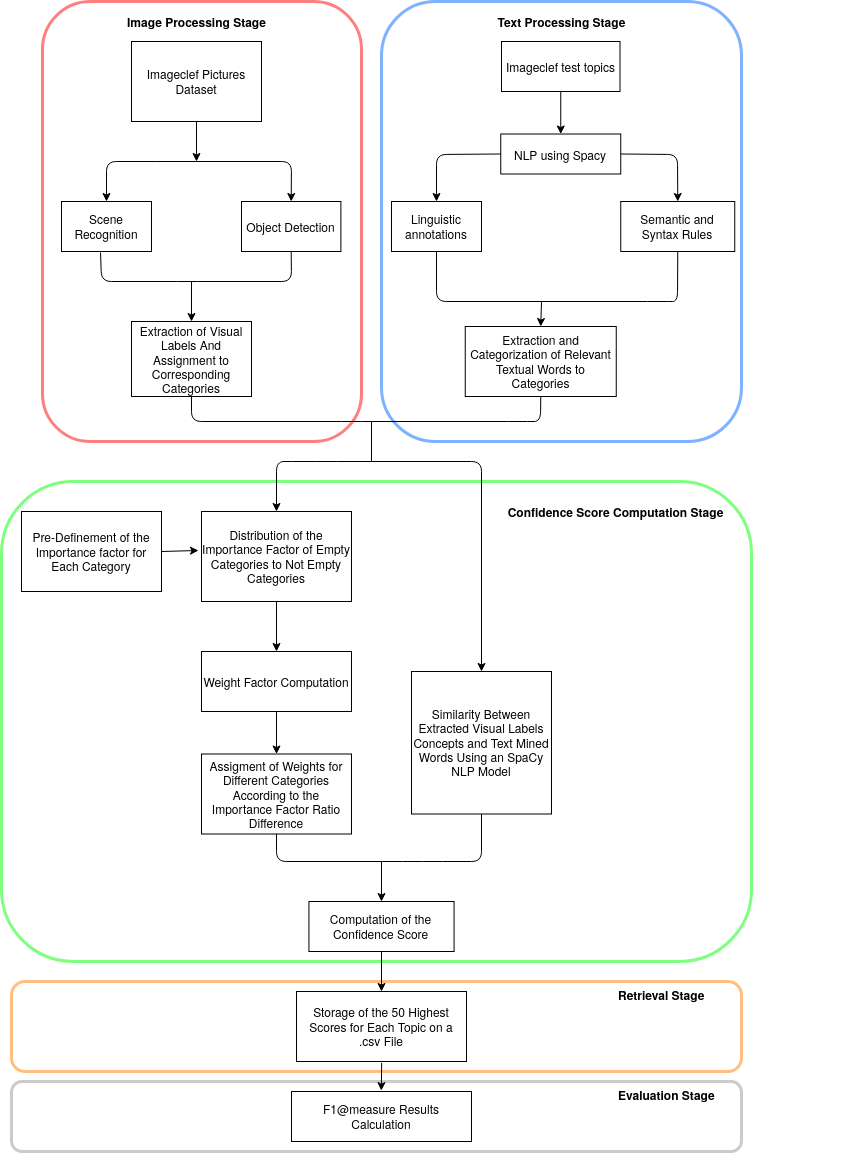
\includegraphics[width = 0.75\textwidth]{Sections/6textprocessing/images/diagram.png}
    \caption{System Architecture}
    \label{fig:testtopic}
  \end{figure}




  